\subsection{Publikum}\label{publikum}

Das Publikum am zentralen Omnibusbahnhof bestand im Wesentlichen aus zwei Gruppen.

Eine Gruppe umfasst die Personen, die wartend an einer Haltestelle auf der ZOB-Insel standen und Blick auf die Installation hatten. Dies waren ab 13:30 Uhr mehrheitlich Schüler.
Zu diesem Zeitpunkt war der ZOB gut gefüllt.
Ab ca. 14:30 Uhr hielten sich hingegen nur noch wenige Passanten an den Haltestellen auf.

Die zweite Gruppe besteht aus Passanten, die zufällig direkt an der Installation vorbeiliefen; mehrheitlich Personen im Alter ab ca. 40 Jahren.

Im Zeitraum von 13:55 Uhr bis 15:05 dokumentierten wir den Durchgangsverkehr vor der Installation, das Verhalten der Passanten und die jeweilige Gruppengröße.
Insgesamt kamen in den 70 Minuten 145 Personen direkt an der Installation vorbei.
112 gingen ohne Reaktion weiter, 31 Personen schauten auf das Display oder in die Wahlkabine (ohne zu Wählen) und 2 Personen gaben jeweils einzeln und unabhängig von einander ihre Stimme ab.
Unter den 145 Personen befanden sich 24 Gruppen á 2 Personen.

\subsubsection{Aktivierungsmuster}\label{aktivierungsmuster}

Während des Experiments fielen uns drei Muster auf, wie Passanten auf die Installation aufmerksam wurden.
Bis auf eine einzige Person haben alle interagierenden Passanten gemeinsam, dass sie nur deshalb interagierten, weil sie auf ihrem Weg sowieso an der Installation vorbeigehen mussten und somit zufällig auf die Wahlkabine oder Display 1
aufmerksam wurden.
Nur eine einzige Person querte zielgerichtet die Straße und wich somit von ihrem eigentlichen Weg ab, um zu partizipieren.

\paragraph{Muster 1: Vorbeigehen \& Schauen}
Das häufigste Interaktionsmuster bestand darin, dass Passanten, die den Gehsteig vor dem Stadt:Raum entlangliefen, die Ergebnisse auf Display 1 betrachteten oder die Wahlkabine beim Vorbeigehen kurz in Augenschein nahmen.
Display 1, dass die Wahlumfrageergebnisse zeigte, verleitete damit Passanten dazu, anzuhalten und sich die Ergebnisse einen Moment anzusehen, bevor sie weitergingen.
Die Wahlkabine diente in diesem Fall als Trigger, der die Aufmerksamkeit auf den Stadt:Raum zog und dadurch womöglich die Wahrnehmung von Display 1 förderte.
Nur wenige Passanten blieben stehen, um die Wahlkabine genauer anzusehen, sondern widmeten ihr im Vorbeigehen ein paar Blicke.
Drei Passanten betraten zwar die Wahlkabine, wählten aber nicht.
Der Großteil der Passanten hat natürlicherweise weder Display 1, noch der Wahlkabine ihre Aufmerksamkeit geschenkt.

\paragraph{Muster 2: Vorbeigehen \& Wählen}
Alle Wähler, bis auf Einen, kamen zufällig an der Wahlkabine vorbei und interagierten infolge dessen.
Keiner der Wähler hat nachträglich auf dem benachbarten Display 1 nachgesehen, wie die Verteilung der Gesamtstimmen ausfällt.
Die Wähler waren alle männlich und mehrheitlich vermutlich über 40 Jahre alt.

\paragraph{Muster 3: Straße queren}
Ein Passant (männlich, ca. 18 Jahre alt) querte vor der Interaktion aktiv die Straße und betrachtete auf Display 1 die Gesamtverteilung der Stimmen.
Er fotografierte das Display mit seinem Smartphone und betrat daraufhin die Wahlkabine, um seine Stimme abzugeben.
Da sich die Wahlentscheidung des jungen Manns mit der Partei mit den zu dieser Zeit meisten Stimmen deckte, mutmaßen wir, dass die Umfrageergebnisse ihn dazu motiviert haben, selbst abzustimmen.


\subsubsection{Interaktion}\label{interaktion}

Während des Deployments waren gleichermaßen vollständig durchgeführte Wahl-Interaktionen (Stimmabgabe ist erfolgt) und unvollständige Wahl-Interaktionen (es wurde versucht, eine Stimme abzugeben, aber es gelang nicht) zu beobachten.

Zwei Seniorinnen hielten sich unabhängig von einander für eine Zeit von 30 bis 60 Sekunden in der Wahlkabine auf, ohne dass eine Stimmabgabe erfasst wurde.
Bei einer der beiden Damen war zu beobachten, dass sie sogar in den Korb mit den Wahlkarten griff.
In Folge dessen war für sie entweder unklar, was sie mit den Wahlkarten tun kann oder sie entschloss sich, nicht zu wählen, weil ihre Partei nicht als Wahlkarte abgebildet war (nur als Option ``Sonstige'').

Ein weiterer Passant (ca. Mitte 40) sprach uns aktiv an, als wir uns gerade in der Nähe der Wahlkabine befanden und fragte, ob er dort seine Stimme für die Bundestagswahl abgeben könne.
Nachdem wir ihm das Experiment erklärt hatten, entschloss sich der Mann, an der Umfrage teilzunehmen.
Er löste die mit einer Schnur an der Installation befestigte Wahlkarte (die Befestigung diente dazu, Diebstahl zu verhindern und sollte gleichzeitig verdeutlichen, dass die Wahlkarte wieder zurückzulegen und nicht einzuwerfen ist) und fragte uns, was damit zu tun ist.
Nachdem wir dem Mann das System erklärt hatten, steckte er die Wahlkarte mehrmals hektisch falsch herum in die Wahlurne und war sich im Unklaren darüber, ob seine Stimme erfasst wurde oder nicht.
Der Mann blickte dabei nicht auf das Display, sondern herunter auf die Wahlurne und konnte so auch nach erfolgreicher Stimmabgabe nicht feststellen, dass seine Stimme registriert wurde.
Wir mutmaßen, dass der Mann das Display vollständig ignorierte, weil er glaubte, bereits alle Informationen von uns erhalten zu haben.
Zudem betonte er mehrmals, dass er sehr in Eile ist (der Mann trug erkennbare Arbeitskleidung).
Auch deshalb hat er sich wahrscheinlich nicht noch einmal die Zeit genommen, die Informationen auf dem Display zu lesen.

Um die Interaktion für die ersten Interessenten zu erleichtern, haben wir am Anfang bereits 10 Stimmen hinzugefügt.
Diese waren zufällig, aber entsprechend der Verteilung der damals aktuellen Umfrageergebnisse, gewählt.
Die folgenden Abbildungen zeigen die abgegebenen Stimmen im Zeitverlauf und das Ergebnisse.
Das unbereinigte Ergebnisse entspricht dem, was am Schluss auf Display 1 zu sehen war, und enthält neben den Seed-Daten auch 2 Instanzen von doppelter Stimmabgabe, bei denen jeweils weniger als 10 Sekunden seit der vorhergehenden Teilnahme vergangen waren.
Zusätzlich waren darin Stimmen enthalten, die wir selbst zur Aufzeichnung unseres Videos abgegeben haben.
All diese Stimmen wurden aus dem bereinigten Ergebnis entfernt, das in Abbildung \ref{fig:result-cleaned} zu sehen ist.

\begin{figure}[ht]
    \centering
    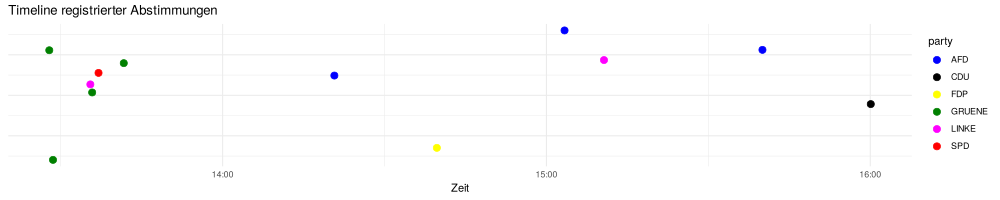
\includegraphics[width=0.8\textwidth]{figures/timeline-cleaned.pdf}
    \caption{Timeline der Interaktionen (bereinigt, siehe Abbildung \ref{fig:result-cleaned})}
    \label{fig:timeline}
\end{figure}

\begin{figure}[ht]
    \centering
    \begin{minipage}{.48\textwidth}
        \centering
        \includegraphics[width=.9\linewidth]{figures/result-all.pdf}
        \captionof{figure}{Abstimmungsergebnis, wie am Ende des Experiments zu sehen}
        \label{fig:result-all}
    \end{minipage}%
    \begin{minipage}{.48\textwidth}
        \centering
        \includegraphics[width=.9\linewidth]{figures/result-cleaned.pdf}
        \captionof{figure}{Abstimmungsergebnis, bereinigt}
        \label{fig:result-cleaned}
    \end{minipage}
\end{figure}